\section{光孤子效应}
\label{sec:optical soliton}
\subsection{孤立波与孤子}
1834 年,英国造船工程师 Russel 骑着马沿着狭窄的运河走时,偶然观察到一个有趣的现象\cite{liangkunmiao}。当小船突然停止前进时,船头会挤出一个水堆。这个水堆保持着自己的形状,以很高的速度沿着河道继续前进。Russel 骑马追了约两英里,它才渐渐消失。Russel 称这种现象为{\bfseries 孤立波(solitary wave)},并在英国科学协会中报告了这一现象,引起了很长时间的争论。

直到 1895 年,两位荷兰的数学家 Korteweg 和 de Vries 在流体动力学的研究中导出了浅水波方程\cite{liangkunmiao},即 KdV 方程
\begin{equation}
    \frac{\partial u}{\partial t}+\alpha u\frac{\partial u}{\partial x}+\frac{\partial^3 u}{\partial x^3}=0
\end{equation}
同时,他们还得到这一方程的一种行波解,在波长趋于无限长的情形下,该行波解能很好地描述 Russel 所发现的孤立波。至此,人们才渐渐接受了 Russel 提出的孤立波的概念,但是这项研究并没有得到人们的广泛关注。

1955 年,Fermi、Pasta 和 Ulam 在一篇有关晶格热传导的论文中提出了一个看似与孤立波无关的问题 —— 在具有非线性相互作用的一维振子链模型中,如果按照能量均分定理,初始能量最终会均分到振子链的所有自由度。但是所得结果却是经过一段时间,能量又基本回到最初的振动模式(FPU 问题)\cite{liangkunmiao}。

一直到 1965 年,美国普林斯顿大学的 Kruskal 和贝尔实验室的 Zabusky 对 FPU 问题进行数值计算。他们发现,在一环形振子链\footnote{周期性边界条件}中,初始脉冲随着时间的推移,演化成几个大小不同的孤立波,它们互相碰撞、穿行,碰撞后仍然保持各自原来的形状与速度,并在某一时刻,所有孤立波在环上同一地点相遇,基本重现初始状态。由于这种类似粒子的性质,Kruskal 和 Zabusky 将这样的孤立波命名为{\bfseries 孤子(soliton)}。{\bfseries 孤子是一种特殊的孤立波,总结其特点\cite{yangbojun,liangkunmiao}
\begin{enumerate}[label=(\arabic*)]
    \item 孤子之间碰撞和相互作用后,能保持其形状和速度不变,仅相位发生变化;
    \item 孤子的能量总是集中在有限的空间区域内,不会耗散到无限的空间区域中去。
\end{enumerate}}

\subsection{孤子本质}
\label{sec:soliton}
目前为止,人们在很多学科领域发现孤子现象,并且在理论上得到了一批描述孤子的非线性偏微分方程(见图\ref{fig:soliton-eq}),孤子问题也逐渐发展为完整、系统的理论。虽然孤子是非线性偏微分方程的一种特殊解,但是孤子的物理本质并不复杂,它是色散效应和非线性效应综合作用的结果。
\begin{figure}[tbp]
    \centering
    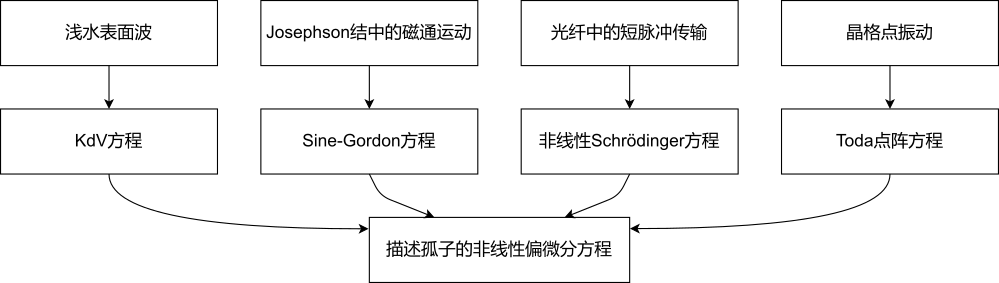
\includegraphics[width=0.9\textwidth]{孤子方程.png}
    \caption{不同领域中的孤子问题}
    \label{fig:soliton-eq}
\end{figure}

不同频率波的传播速度不同形成色散,色散使脉冲(波包)在传输过程中逐渐展宽,能量逐渐耗散,最终导致脉冲(波包)消失;非线性波的传播速度依赖于振幅,振幅越大的地方传播速度越快,这就使得波的前沿不断变陡,波形更加尖锐。{\bfseries 因此,色散作用使波形平展,非线性效应使波形尖锐,两者的作用刚好相反。当两种因素相互平衡时,便能使波形保持不变,形成孤子\cite{liangkunmiao}。}

如\ref{sec:Schrodinger}节所述,非线性 Schr\"odinger 方程描述的就是色散效应和非线性效应共同作用下脉冲在光纤中的传输过程。Hasegawa 和 Tappert 就在 1973 年指出,反常群速度色散和非线性效应的相互作用使得孤子脉冲可以在低损光纤中传输,并通过数值实验证实了光孤子在通信系统中的稳定性\cite{Hasegawa}。

为了描述到底是色散效应还是非线性效应对脉冲的传输演化起主要作用,需要对非线性 Schr\"odinger 方程进行无量纲化处理,并引入色散长度 $L_D$ 和非线性长度 $L_{NL}$ 来衡量脉冲传输过程中色散和非线性效应哪个起重要作用。那么,先对脉冲进行归一化处理
\begin{align}
    &\tau=\frac{T}{T_0}=\frac{t-z/v_g}{T_0} \nonumber \\
    &A(z,\tau)=\sqrt{P_0}U(z,\tau)
\end{align}
$T_0$ 为初始脉宽,$\tau$ 是归一化时间尺度(不具有时间量纲),$P_0$ 为入射脉冲峰值功率,$U$ 是归一化振幅(也不具备振幅量纲),已忽略光纤的损耗系数 $\alpha$。根据非线性 Schr\"odinger 方程(\ref{eq:Schrodinger}), 归一化振幅 $U(z,\tau)$ 需满足
\begin{align}
    i\frac{\partial U}{\partial z}&=\frac{\mathrm{sng}(\beta_2)}{2L_D}\frac{\partial^2U}{\partial \tau^2}-\frac{1}{L_{NL}}|U|^2U\\
    L_D&=\frac{T^2_0}{|\beta_2|}\hspace{4ex}L_{NL}=\frac{1}{\gamma P_0} \nonumber
\end{align}

可根据脉冲传输距离 $z$ 与色散长度 $L_D$ 和非线性长度 $L_{NL}$ 之间的相对大小,将光纤分为不同的传输区域\cite{Agrawal}
\begin{enumerate}[label=(\arabic*)]
    \item $z\ll L_{D}$ 且 $z\ll L_{NL}$,色散和非线性效应都不起重要作用。传输过程中,脉冲形状保持不变(见图\ref{fig:distortionless})。
    \item $z\ll L_{NL}$ 而 $z\approx L_{D}$,脉冲传输演化过程中,群速度色散(GVD)起主要作用,使脉冲展宽(见图\ref{fig:GVD})。
    \item $z\ll L_{D}$ 但 $z\approx L_{NL}$,非线性效应对脉冲起主要作用。其结果是产生自相位调制(self-phase modulation,SPM)现象,使脉冲频谱发生变化。较强的自相位调制和较弱的群速度色散导致光波分裂现象,脉冲前后沿变陡,并演化出快速振荡的精细结构(见图\ref{fig:SPM_time}),频谱中央也因此产生多峰结构\cite{Agrawal}(见图\ref{fig:SPM_frequent})。
    \item $z\approx L_{D}$,$z\approx L_{NL}$,色散和非线性效应对脉冲传输都有重要作用。在正常色散区 $\beta_2>0$,群速度色散和自相位调制可用于脉冲压缩;在反常色散区 $\beta_2<0$,两者的作用能形成光孤子\cite{Agrawal}。
\end{enumerate}
\begin{figure}[tbp]
    \centering
    \begin{minipage}[t]{0.45\linewidth}
        \centering
        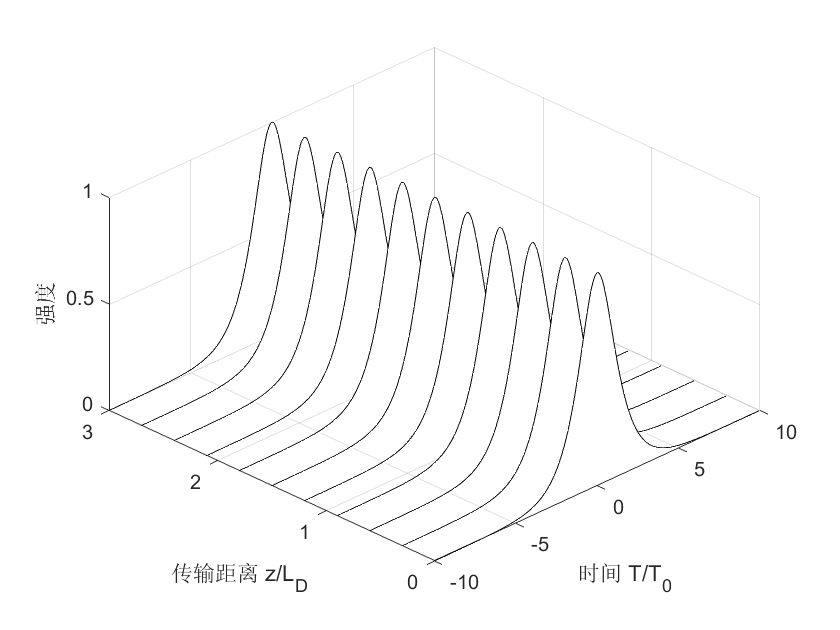
\includegraphics[width=1\linewidth]{脉冲无畸变传输.png}
        \caption{脉冲无畸变传输}
        \label{fig:distortionless}
    \end{minipage}       
    \begin{minipage}[t]{0.45\linewidth}
        \centering
        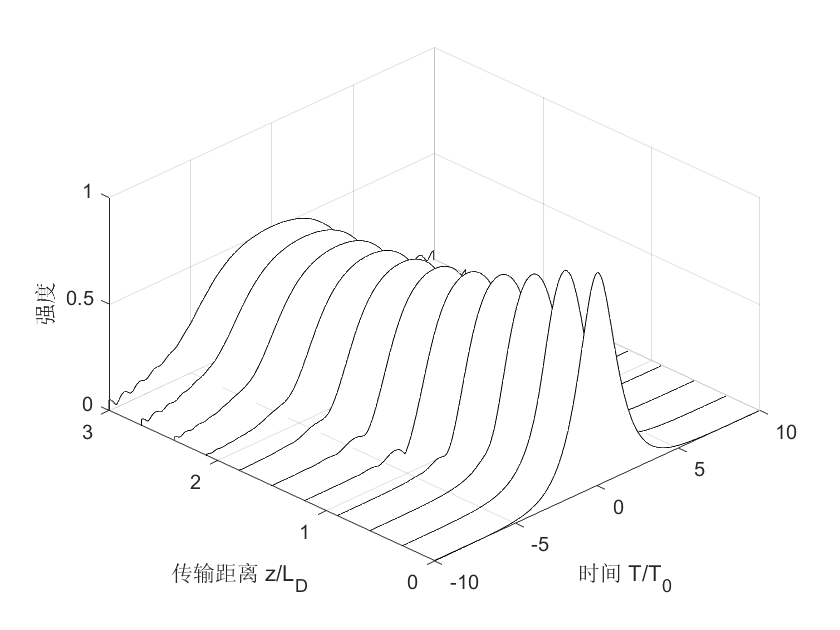
\includegraphics[width=1\linewidth]{脉冲展宽.png}
        \caption{群速度色散导致脉冲展宽}
        \label{fig:GVD}    
    \end{minipage}
\end{figure}
\begin{figure}[tbp]
    \centering
    \begin{subfigure}[t]{0.45\linewidth}
        \begin{minipage}[b]{1\linewidth}
        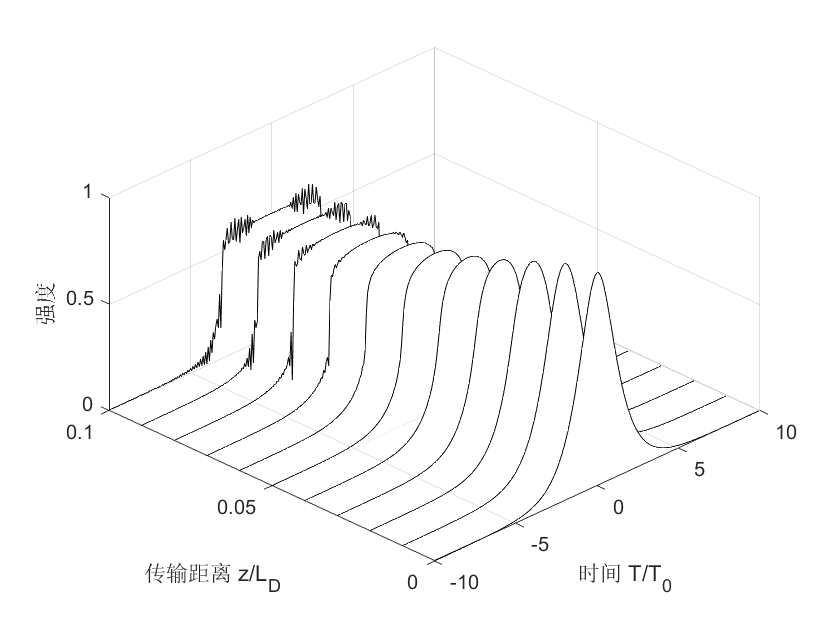
\includegraphics[width=1\linewidth]{自相位调制_时域.png}
        \caption{时域}
        \label{fig:SPM_time}
        \end{minipage}
    \end{subfigure}
    \begin{subfigure}[t]{0.45\linewidth}
        \begin{minipage}[b]{1\linewidth}
        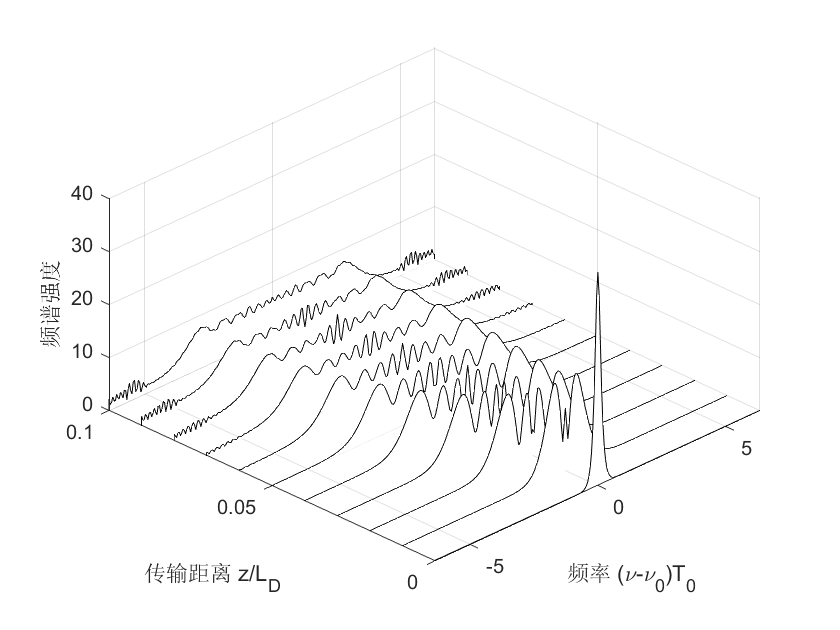
\includegraphics[width=1\linewidth]{自相位调制_频域.png}
        \caption{频域}
        \label{fig:SPM_frequent}
        \end{minipage}
    \end{subfigure}
    \caption{自相位调制主要影响下的光波分裂}
\end{figure}

\subsection{逆散射方法}
如 \ref{sec:soliton} 节所述,孤子现象由一些特殊的非线性偏微分方程所描述,人们在研究这些特殊的非线性偏微分方程的过程中发展了量子力学中的逆散射方法(the Inverse Scattering Transform Method,简称 IST)。

1967 年,Gardner 等人将 IST 方法应用于 KdV 方程求解,对孤子现象做出严格的数学证明。一开始,人们认为 IST 方法能用于求解 KdV 方程仅仅是因为 Schr\"odinger 方程与 KdV 方程之间的巧妙联系。但是,Lax 在 1968 年对 IST 方法做了推广,使得 IST 方法能求解更多的非线性偏微分方程。1971 年,Zakharov 和 Shabat 将 IST 方法用于非线性 Schr\"odinger 方程的求解,并给出了非线性 Schr\"odinger 方程的解析解\cite{yangbojun,Zakharov}。

量子力学中,Schr\"dinger 方程的散射问题是根据已知势场求解散射数据以及波函数在无穷远处的渐近行为;逆散射问题正好相反,已知散射数据和波函数在无穷远处的边界条件反向求解散射势\footnote{逆散射方法最初就是利用散射数据来构造势能曲线,以了解原子与分子结构。}。{\bfseries IST 方法并不是直接去求非线性偏微分方程的解,而是把非线性演化问题作为一个散射问题考虑,根据初始散射数据求解散射数据在散射过程中的演化,再由演化的散射数据重构位势,散射势就是非线性偏微分方程的解。IST 方法的思想与 Fourier 变换法求解线性偏微分方程非常类似(见图\ref{fig:Fourier}),因此 IST 方法也常被称为非线性 Fourier 变换法\cite{liangkunmiao}。}
\begin{figure}[tbp]
    \centering
    \begin{subfigure}[t]{0.40\linewidth}
        \begin{minipage}[b]{1\linewidth}
        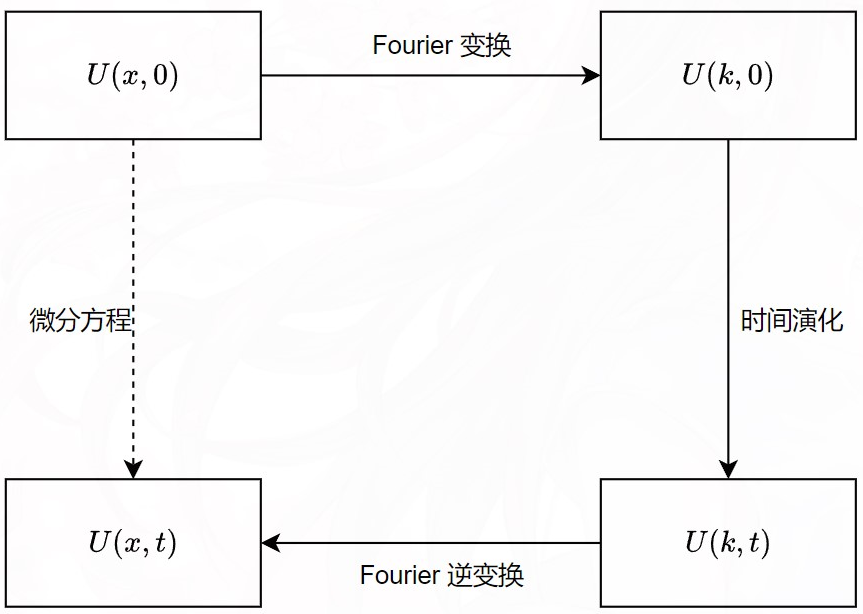
\includegraphics[width=1\linewidth]{线性傅里叶变换.png}
        \caption{线性Fourier变换法}
        \label{fig:Fourier_pde}
        \end{minipage}
    \end{subfigure}
    \hspace{4ex}
    \begin{subfigure}[t]{0.40\linewidth}
        \begin{minipage}[b]{1\linewidth}
        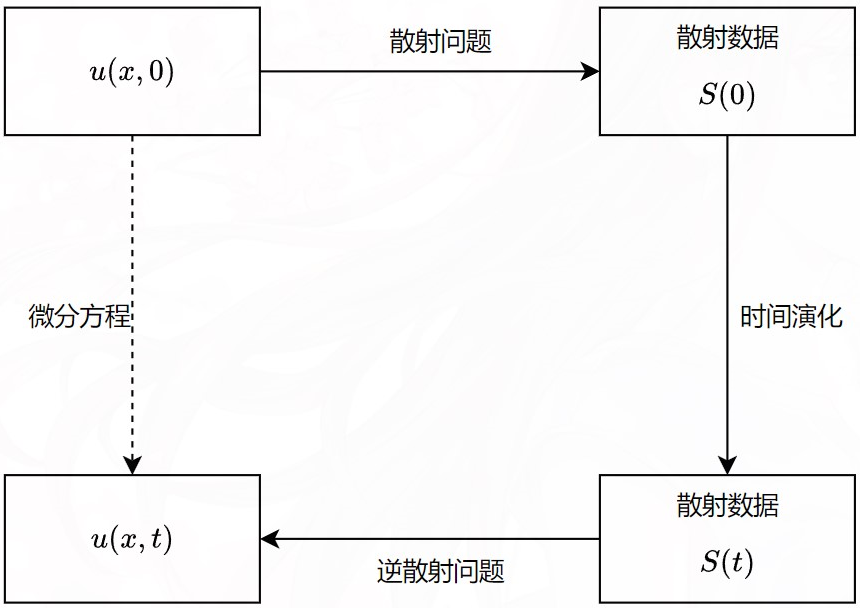
\includegraphics[width=1\linewidth]{非线性傅里叶变换.png}
        \caption{非线性Fourier变换法}
        \end{minipage}
    \end{subfigure}
    \caption{Fourier变换方法与逆散射方法}
    \label{fig:Fourier}
\end{figure}

本节着重讨论非线性 Schr\"odinger 方程的 IST 方法求解。不妨对传输距离 $z$ 也做无量纲化处理 $\xi=z/L_D$,并引入参量 $N^2=L_{D}/L_{NL}$,把非线性 Schr\"odinger 表述成更简洁的形式
\begin{equation}
    i\frac{\partial U}{\partial \xi}=\mathrm{sng}(\beta_2)\frac{1}{2}\frac{\partial^2 U}{\partial \tau^2}-N^2|U|^2U
\end{equation}
在反常色散区 $\beta_2<0$,标准化的非线性 Schr\"odinger 方程为
\begin{align}
    &u=NU=\sqrt{\gamma L_D} A\nonumber \\
    &i\frac{\partial u}{\partial \xi}+\frac{1}{2}\frac{\partial^2 u}{\partial \tau^2}+|u|^2u=0
    \label{eq:NLSE}
\end{align}
与该非线性演化相联系的散射问题是\cite{guoyucui}
\begin{equation}
    \begin{pmatrix}
        i\partial/\partial \tau & u \\
        -u^* & -i\partial/\partial \tau
    \end{pmatrix}\begin{bmatrix}
        \psi_1\\
        \psi_2
    \end{bmatrix}=k\begin{bmatrix}
        \psi_1\\
        \psi_2
    \end{bmatrix}
    \label{eq:scatter}
\end{equation}
其中,$\psi_1$ 和 $\psi_2$ 是被势场 $u(\xi,\tau)$ 散射的两个波函数,$k$ 是本征值。根据 Lax 推广的 IST 方法,非线性偏微分方程应等价为两个线性问题,其中一个就是如(\ref{eq:scatter})所示的散射问题;另一个线性方程描述波函数随空间传输的演化过程
\begin{equation}
    \frac{\partial}{\partial \xi}\begin{bmatrix}
        \psi_1\\
        \psi_2
    \end{bmatrix}=\textbf{\textit{M}}\begin{bmatrix}
        \psi_1\\
        \psi_2
    \end{bmatrix}
    \label{eq:wave function evolution}
\end{equation}
算子 $\textbf{\textit{M}}$ 的具体形式需要用 AKNS 方法\footnote{1973 年,Ablowitz、Kaup、Newell 和 Segur 在求解 Sine-Gordon 方程时提出由散射问题算子 $\hat{L}$ 构造波函数演化算子 $\hat{M}$ 的方法}推导\cite{guoyucui},结果比较繁琐,此处不再说明。

散射问题(\ref{eq:scatter})是一个本征值问题。{\bfseries 当本征值 $k$ 为实数时,可以取连续值,本征函数为行波解,即波函数对应于连续态},其在无穷远处的渐进行为
\begin{equation}
    \begin{bmatrix}
        \psi_1\\
        \psi_2
    \end{bmatrix}=\left\{\begin{aligned}
        &\begin{bmatrix}
            1\\
            0
        \end{bmatrix}e^{-ik\tau}+R(k,\xi)\begin{bmatrix}
            0\\
            1
        \end{bmatrix}e^{ik\tau}, & \tau\to-\infty\\
        &T(k,\xi)\begin{bmatrix}
            1\\
            0
        \end{bmatrix}e^{-ik\xi}, & \tau\to\infty
    \end{aligned}\right.
\end{equation}
其中,$R(k,\xi)$ 为反射系数,$T(k,\xi)$ 为透射系数。{\bfseries 当本征值 $k$ 为复数时,只能取有限个分立值 $k_n$,本征函数指数衰减,即波函数对应为束缚态(孤子)}。这种情形下,本征值 $k_n$ 正是反射系数 $R(k,\xi)$ 在 $k$ 平面上的极点,对应的留数为 $C_{n}(k_n,\xi)$\cite{guoyucui}。

连续本征值 $k$ 对应的反射系数 $R(k,\xi)$ 和离散本征值 $k_n$ 对应的留数 $C(k_n,\xi)$ 就是散射问题(\ref{eq:scatter})的散射数据。可由波函数演化方程(\ref{eq:wave function evolution})确定散射数据随传输距离的演化关系
\begin{subequations}
    \begin{align}
        R(k,\xi)&=R(k,0)e^{i2k^2\xi}\\
        C_n(k_n,\xi)&=C_n(k_n,0)e^{ik_n^2\xi}
    \end{align}
\end{subequations}


根据 $\xi=0$ 处的输入脉冲得到初始的散射数据 $R(k,0)$ 和 $C_n(k_n,0)$\footnote{1974 年,Satsuma 和 Yajima 讨论了初始条件对非线性 Schr\"odinger 方程解的影响。},脉冲在光纤中的传输对应于散射数据演化,直接给出逆散射问题的结果,也就是散射势
\begin{equation}
    u(\xi,\tau)=-2K_1(\tau,\tau,\xi)
\end{equation}
其中,函数 $K_1(x,y,t)$ 满足 Gel'fand-Levitan-Marchenko 积分方程(简称 GLM 方程)
\begin{equation}
    \left\{\begin{aligned}
        &K_1(x,y,t)=B^*(x+y,t)+\int_x^\infty B^*(y+z,t)K_2^*(x,z,t)\mathrm{d}z\\
        &K_2^*(x,y,t)=-\int_x^\infty B(y+z,t)K_1(x,z)\mathrm{d}z
    \end{aligned}\right.
    \label{eq:GLM}
\end{equation}
积分核 $B(x+y,\xi)$ 由散射数据给出
\begin{equation}
    B(x+y,\xi)=\sum_{n=1}^NC^2_n(ik_n,\xi)e^{k_n(x+y)}+\frac{1}{2\pi}\int_{-\infty}^{\infty}R(k,\xi)e^{ik(x+y)}\mathrm{d}k
\end{equation}

上述过程给出了严格求解非线性 Schrodinger 方程的步骤,其中不可避免地要求解复杂的积分方程(\ref{eq:GLM})。但是,对于无反射的孤子解情形 $R(k,0)=0$,便可通过求解代数方程组得到 $u(\xi,\tau)$
\begin{align}
    u(\xi,\tau)&=-2\sum_{n=1}^{N}\lambda_n^*\psi_{2n}^* 
    \label{eq:soliton}\\
    \lambda_n^*&=\sqrt{C_n}e^{i(k_n\tau+k_n^2\xi)} \nonumber
\end{align}
其中,$\psi_{2n}^*$ 满足代数方程组
\begin{equation}
    \begin{aligned}
        \psi_{1n}+\sum_{n'=1}^N\frac{\lambda_n\lambda_{n'}^*}{k_n-k^*_{n'}}\psi^*_{2n'}&=0\\
        \psi_{2n}^*-\sum_{n'=1}^N\frac{\lambda^*_{n}\lambda_{n'}}{k^*_n-k_{n'}}\psi_{1n'}&=\lambda_n^*
    \end{aligned}
\end{equation}
极点数目 $N$ 或离散本征值 $k_n$ 的数目表征孤子阶数。
\subsection{光孤子}
从 IST 方法求解非线性 Schr\"odinger 方程的过程我们清楚地可以知道,光孤子解来自散射问题的束缚态($R(k,\xi)$ 的极点处,本征值为复数 $k_n$)。上一节仅在反常群速度色散区讨论光孤子的解,随着光纤和激光技术的成熟,人们在实验上发现或者在理论上提出了多种光孤子(见图\ref{fig:optical soliton}),本文重点讨论反常色散区的光孤子(亮孤子)\cite{Agrawal}。
\begin{figure}[hbtp]
    \centering
    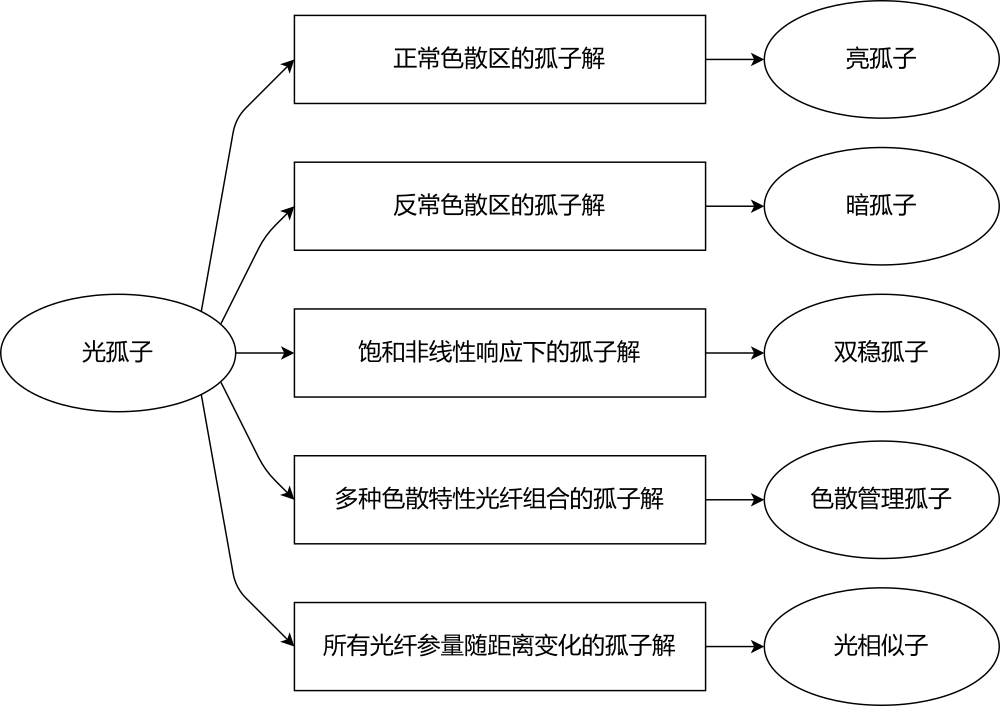
\includegraphics[width=0.6\textwidth]{光孤子.png}
    \caption{不同类型的光孤子}
    \label{fig:optical soliton}
\end{figure}
\subsubsection{基阶孤子}
单个本征值 $N=1$ 的情形下,脉冲传输能形成基阶孤子,可通过求解孤子解方程组(\ref{eq:soliton})得到基阶孤子的一般形式
\begin{equation}
    u(\xi,\tau)=\eta\mathrm{sech}[\eta(\tau-\tau_s+\delta\xi)]\exp[i(\eta^2-\delta^2)\xi/2-i\delta\tau+i\phi_s]
\end{equation}
其中,$\eta$、$\delta$、$\tau_s$ 和 $\phi_s$ 是表征基阶孤子的 4 个参数。$\phi_s$ 是相位常数,在研究单孤子问题时常把它忽略,在讨论孤子相互作用问题时才起作用。参量 $\tau_s$ 表示孤子峰的位置,选取适当的时间原点可以使 $\tau_s=0$。参量 $\eta$ 不仅决定孤子的振幅,而且同时决定了孤子的宽度。参量 $\delta$ 表示孤子相对于中心频率 $\omega_0$ 的频移,同时也导致群速度 $v_g$ 的改变\cite{Agrawal}
\begin{equation}
    \begin{aligned}
        |u(\xi,\tau)|&=\eta\mathrm{sech}[\eta(\tau+\delta\xi)]=\eta\mathrm{sech}\left[\eta\left(\frac{t-\beta_1z}{T_0}+\delta\frac{z}{L_D}\right)\right]\\
        &=\eta\mathrm{sech}\left(\eta\frac{t-\beta'_1z}{T_0}\right)\\
        \beta'_1&=\beta_1-\frac{\delta|\beta_2|}{T_0}
    \end{aligned}
\end{equation}

在忽略相位常量 $\phi_s$、孤子中心 $\tau_s$ 和频移 $\delta$ 参量后,基阶孤子可以描述为
\begin{equation}
    u(\xi,\tau)=\eta\mathrm{sech}(\eta\tau)\exp\left(i\frac{\eta^2\xi}{2}\right)
\end{equation}
从中我们可以发现
\begin{enumerate}[label=(\arabic*)]
    \item 孤子宽度 $T_0/\eta$ 反比于孤子振幅 $\eta$,这是孤子很重要的一个特点;
    \item 对于 $N=1$ 的基阶孤子脉冲,在光纤中将无畸变地传输(见图\ref{fig:first soliton}),这使得基阶孤子在光纤通信中具有广阔前景。
\end{enumerate}
\begin{figure}[bp]
    \centering
    \begin{minipage}[t]{0.45\linewidth}
        \centering
        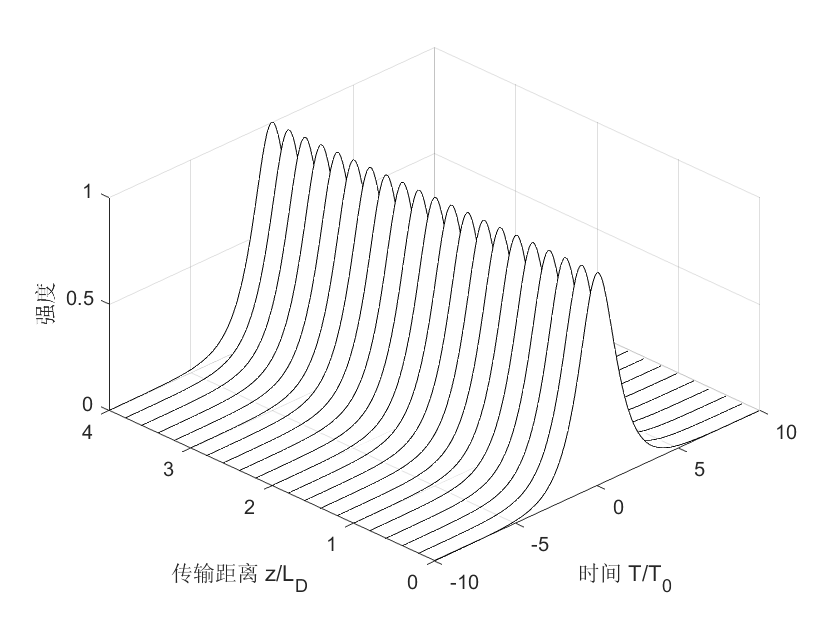
\includegraphics[width=1\linewidth]{基阶孤子无畸变传输.png}
        \caption{基阶孤子无畸变传输}
        \label{fig:first soliton}
    \end{minipage}       
    \begin{minipage}[t]{0.45\linewidth}
        \centering
        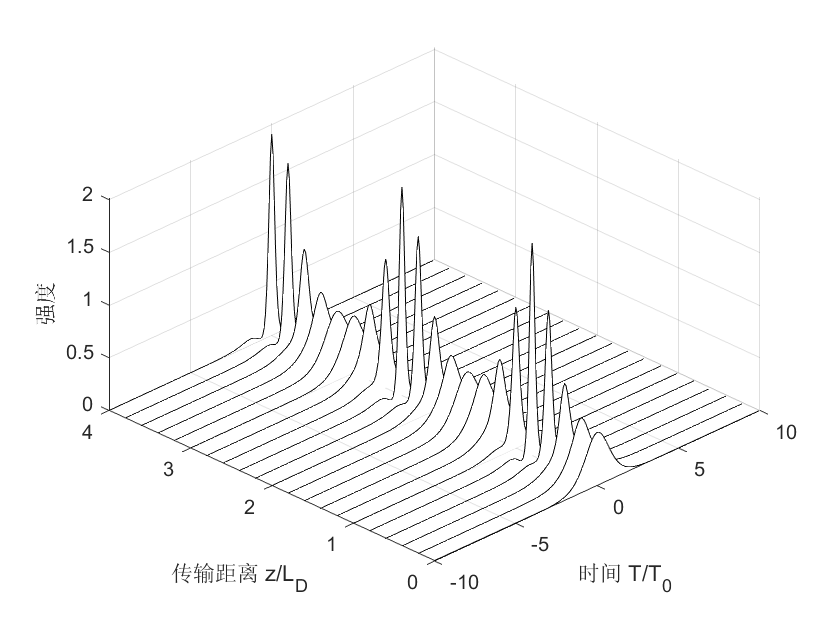
\includegraphics[width=1\linewidth]{二阶孤子解析解.png}
        \caption{二阶孤子的周期性演化}
        \label{fig:second soliton}    
    \end{minipage}
\end{figure}
\subsubsection{二阶和高阶孤子}
高阶孤子也可以用通解(\ref{eq:soliton})来描述,不同的本征值 $k_n$ 和留数 $C_n$ 可以构造出各种各样的高阶孤子。可根据本征值与留数的关系区分不同的孤子集,其中一类孤子集其初始形状如下
\begin{equation}
    u(0,\tau)=N\mathrm{sech}(\tau)
\end{equation}
孤子阶数 $N$ 为整数\footnote{当 $N$ 不为整数时,涉及到孤子稳定性问题,本文不做讨论。}。这一类孤子有一个很有趣的特征——包络形状 $|u(\xi,\tau)|$ 做周期 $\xi_0=\pi/2$ 的周期性变化。拿二阶孤子举例,对于本征值 $k_1=1/2$ 和 $k_2=3i/2$ 的二阶孤子,其场分布 $u(\xi,\tau)$
\begin{equation}
    u(\xi,\tau)=\frac{4[\cosh(3\tau)+3e^{4i\xi}\cosh(\tau)]}{\cosh(4\tau)+4\cosh(2\tau)+3\cos(4\xi)}e^{i\xi/2}
\end{equation}
根据场分布 $u(\xi,\tau)$ 的解析表达式作图(见图\ref{fig:second soliton}),可以发现孤子周期 $z_0$
\begin{equation}
    z_0=\xi_0L_D=\frac{\pi}{2}\frac{T^2_0}{|\beta_2|^2}
\end{equation}

对三阶孤子($N=3$)进行数值模拟(见图\ref{fig:third soliton_time})。发现脉冲在光纤中传输时,开始阶段脉宽被压缩,在 $z_0/2$ 处被窄化的脉冲一分为二,在孤子周期 $z_0$ 处又变回原来形状的单个脉冲。脉冲变窄、分裂、再恢复的过程在每个孤子周期内重复进行。

从三阶孤子的频谱演化过程来看(见图\ref{fig:third soliton_frequent}),在 $z=0.3L_D$ 附近,出现了自相位调制的典型振荡结构,这种振荡性的频谱结构使得孤子的前沿和后沿发生变化,导致脉冲分裂;随后的反常群速度色散导致脉宽变窄,脉冲频谱也相应改变。也就是说,自相位调制和群速度色散交替的主导作用使得光孤子无论是时域还是频域上来看都将呈现周期性的演化过程\cite{Agrawal}。
\begin{figure}[btp]
    \centering
    \begin{subfigure}[t]{0.45\linewidth}
        \begin{minipage}[b]{1\linewidth}
        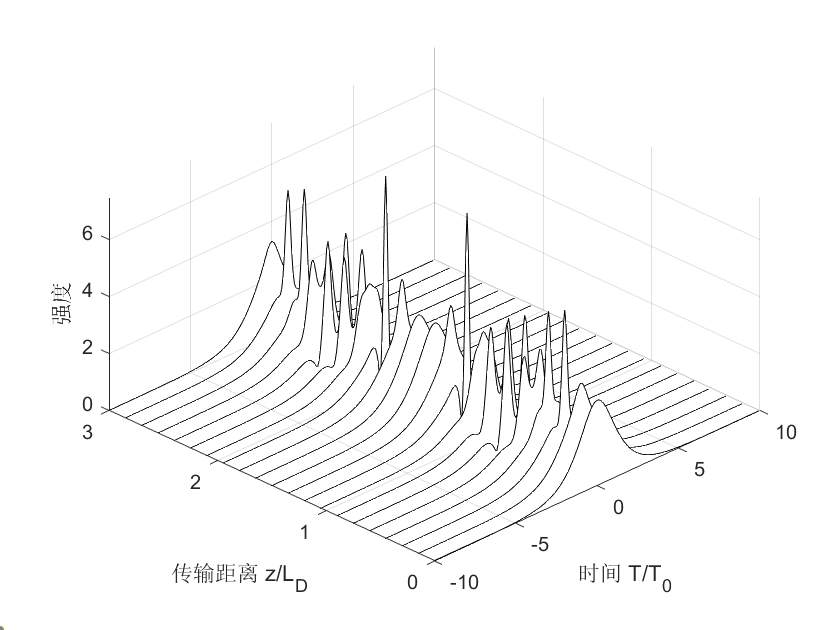
\includegraphics[width=1\linewidth]{三阶孤子演化_时域.png}
        \caption{时域}
        \label{fig:third soliton_time}
        \end{minipage}
    \end{subfigure}
    \begin{subfigure}[t]{0.45\linewidth}
        \begin{minipage}[b]{1\linewidth}
        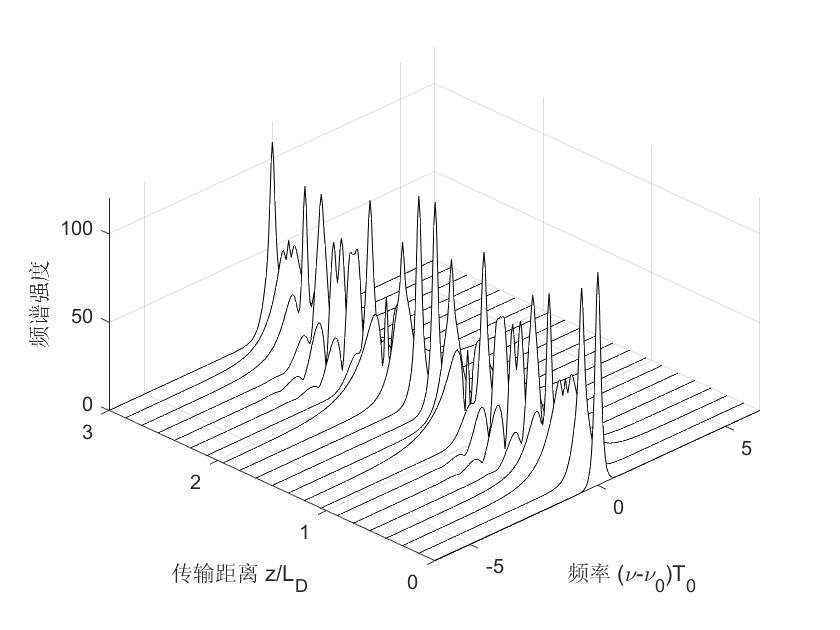
\includegraphics[width=1\linewidth]{三阶孤子演化_频域.png}
        \caption{频域}
        \label{fig:third soliton_frequent}    
        \end{minipage}
    \end{subfigure}
    \caption{三阶孤子的周期性演化}
\end{figure}

{\bfseries 对于基阶孤子($N=1$),自相位调制和色散影响互相平衡,脉冲的形状和频谱几乎不随传输变化。对于二阶、三阶甚至更高阶的孤子,自相位调制和群速度色散的影响地位是交替变化着的,导致传输过程中出现脉冲变窄、分裂、再恢复的周期性演化结果\cite{Agrawal}。}